\documentclass{report}

\usepackage{geometry}
\geometry{margin=1in}

\usepackage{amsmath}
\usepackage{amssymb}

\usepackage{graphicx}
\graphicspath{}

\DeclareMathOperator*{\argmax}{arg\,max}

\title{STAT 672: Homework 2}

\author{Tom Wallace}

\begin{document}

\maketitle

\section*{Problem 1}

\subsection*{A}

For a supervised learning problem, risk is defined as the expected value
of the loss function:
$$
R(f) = \mathbf{E}_{X, Y \sim P}[L(Y, f(x))]
$$
Bayes risk is the risk present when using the Bayes classifier $f^*(x)$:
$$f^*(x) = \argmax_Y P(Y=y|X=x)$$
Typically, this classifier is not practical because we do not know the
conditional distribution of $Y$ given $X$, but in this problem it is given.
Our resultant Bayes classifier is:
$$
f^*(x) = 
\begin{cases}
0 & x \in [0.2, 0.8] \\
1 & x \in \{(0, 0.2) \cup (0.8, 1)\} 
\end{cases}
$$
Suppose that we use a typical 0-1 loss function.  
$$
L(y, f(x)) = 
\begin{cases} 
	0 & y = \mathrm{sign}(f(x)) \\ 
	1 & \mathrm{otherwise}
\end{cases}
$$
Risk in our problem is equal to:
$$
P(\mathrm{sign}(Y) \neq \mathrm{sign}(f(x)))
$$
Using the law of total probability, this is equal to:
\begin{equation}
	\begin{split}
	& P(Y=0|X \in \{(0, 0.2) \cup (0.8, 1)\})P(X \in \{(0, 0.2) \cup (0.8,
	1)\}) \\
	& + P(Y=1|X \in [0.2, 0.8])P(X \in [0.2, 0.8]) 
	\end{split}
\end{equation}

$$
(0.2 \times 0.1) + (0.2 \times 0.1) + (0.2 \times 0.6) = 0.16
$$

\subsection*{B}
First, consider $d=0$. $f(x)$ must take the form of $f(x) =
C$, with $C$ being some constant. Because $Y \in \{-1, 1\}$, our candidate functions are $f(x)
= 1$ (i.e. always predict that $Y=1$, regardless of $x$) and $f(x) = -1$ (i.e.
always predict that $Y=-1$, regardless of $x$). We calculate the risk for each:

\begin{equation*}
	\begin{split}
		R(f(x)) = & P(Y \neq 1 | X\in(0, 0.2))P(X\in(0, 0.2)) \\
		  & + P(Y \neq 1 | X\in[0.2, 0.8])P(X\in[0.2, 0.8]) \\ 
		  & + P(Y \neq 1 | X\in(0.8, 1))P(X\in(0.8, 1))
	\end{split}
\end{equation*}
$$
=(0.1)(0.2) + (0.8)(0.6) + (0.1)(0.2) = 0.52
$$
By similar logic, $R(f(x)=-1) = 0.48$. This is smaller than $0.52$ and so is the
best we can do for $d=0$. Excess risk for $d=0$ is:
$$
\min_{f \in \mathcal{F}_{d=0}} R(f) - R(f^*) = 0.48 - 0.16 = 0.32
$$
Lastly, consider $d=1$. Our candidate functions are of the form:
$$
f(x) = \alpha x + C
$$
This equation defines a straight line and so we are limited to a
``threshold'' approach: for example, always predict that $Y=1$ if $x$ is greater
than some value. Because the distribution of $Y|X$ is a simple step function, we
have some obvious candidate functions. Consider 
$f(x)=-x+0.2$, i.e. predict that $Y=1$ for
$X \in (0, 0.2)$ and $Y=-1$ for $X\in(0.2, 0.8)$:

\begin{equation*}
	\begin{split}
		R(f(x)) = & P(Y \neq 1  | X\in(0, 0.2))P(X\in(0, 0.2))  \\
		  & + P(Y \neq -1  | X\in(0.2, 0.8))P(X\in(0.2, 0.8))  \\ 
		  & + P(Y \neq -1 | X\in(0.8, 1.0))P(X\in(0.8,1.0)) 
	\end{split}
\end{equation*}
$$
= (0.1)(0.2) + (0.6)(0.2) + (0.9)(0.2) = 0.32
$$
By symmetry the risk of this function is the same as
other similar candidates that set the threshold at a discontinuity in the step
function: we cannot do better. Excess risk for $d=1$ thus is:
$$
\min_{f \in \mathcal{F}_{d=1}} R(f) - R(f^*) = 0.32 - 0.16 = 0.16
$$
Lastly, consider $d=2$. Our candidate functions are of the form:
$$
f(x) = \alpha_1 x^2 + \alpha_2 x + C
$$
A good candidate is $f(x)=(x-0.2)(x-0.8)$. This function will return a positive
number (i.e., predict that $Y=1$) if $x \in (0, 0.2)$, and will return a
negative number (i.e., predict that $Y=-1$) if $x \in (0.2, 0.8)$. Risk is thus
equal to:

\begin{equation*}
	\begin{split}
		R(f(x)) = & P(Y \neq 1  | X\in(0, 0.2))P(X\in(0, 0.2))  \\
		  & + P(Y \neq -1  | X\in(0.2, 0.8))P(X\in(0.2, 0.8))  \\ 
		  & + P(Y \neq 1 | X\in(0.8, 1.0))P(X\in(0.8,1.0)) 
	\end{split}
\end{equation*}
$$
(0.2)(0.1) + (0.2)(0.1) + (0.2)(0.6) = 0.16
$$
And excess risk is:
$$
\min_{f \in \mathcal{F}_{d=2}} R(f) - R(f^*) = 0.16 - 0.16 = 0
$$
Further increasing dimensionality ($d=3, 4\ldots$) will allow
us to do as well (i.e. achieve zero excess risk) but no better, since Bayes
risk is the theoretical optimum. We have proved the following two statements 
and so can conclude that excess risk is zero if and only if $d \geq 2$:

\begin{itemize}
	\item $\min_{f \in \mathcal{F}_{d \geq 2}} R(f) - R(f^*) = 0$ \qquad (if)
	\item $\min_{f \in \mathcal{F}_{d<2}} R(f) - R(f^*) > 0$ \qquad (only
		if)
\end{itemize}

\newpage

\subsection*{C}

See \texttt{hw2.py}. I empirically tested the accuracy of my $X$ and $Y|X$
generating functions by generating 10,000 observations with them and plotting the results,
as seen in Figure 1. Although this is just a crude 10-bin histogram 
and so does not perfectly match the theoretical distribution, it appears broadly
correct; for example, it has a ``barbell'' shape.

\begin{figure}[h]
	\caption{Problem 1-C Generating Functions}
	\centering
	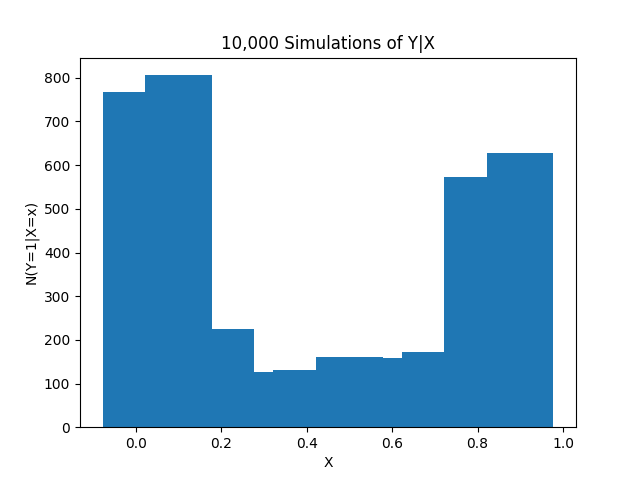
\includegraphics[scale=0.5]{hist}
\end{figure}

\subsection*{D}

See \texttt{hw2.py}. TALK ABOUT FUNCTIONS.

\subsection*{E}

Advanced simulation

\end{document}
